\pdfoutput=1
\documentclass[preview]{standalone}

\usepackage[utf8]{inputenc}
\usepackage{lmodern}
\usepackage[T1]{fontenc}

\usepackage{verbatim}
\usepackage{graphicx}
	\DeclareGraphicsRule{*}{mps}{*}{}
\usepackage{xcolor}

\usepackage{tikz}
	\usetikzlibrary{calc}
	\usetikzlibrary{arrows}
	\usetikzlibrary{backgrounds}
	\usetikzlibrary{decorations.pathmorphing}
	\usetikzlibrary{shapes.geometric}
	\tikzset{>=latex'}

\usepackage{amsmath}
\usepackage{amssymb}
\usepackage{dsfont}
\usepackage{nicefrac}
\usepackage{mathrsfs}
\usepackage[Euler]{upgreek}
\usepackage[nointegrals]{wasysym}
\usepackage{booktabs}
\usepackage{float}

\begin{document}

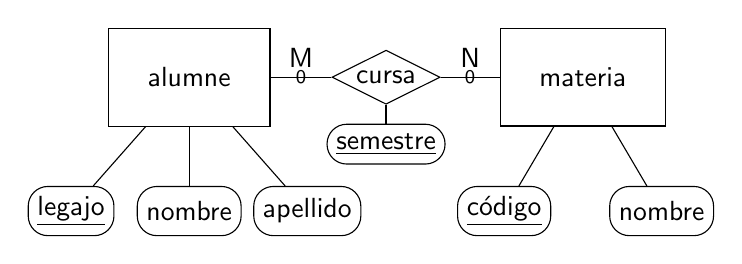
\begin{tikzpicture}[font=\sffamily]
	\node[draw,inner sep=5mm] (alumne) at (0,0) {alumne};
	\node[draw,inner sep=5mm] (materia) at (5,0) {materia};
	\node[draw,shape aspect=2,diamond,inner sep=0.5mm] (cursa) at (2.5,0) {cursa};
	\draw (alumne) -- node[above]{M} node{\scriptsize 0} (cursa) -- node[above]{N} node{\scriptsize 0} (materia);
	\node[draw,rounded corners=2.5mm,minimum height=6.25mm] (legajo) at (-1.5,-1.7) {$\underline{\text{legajo}}$};
	\node[draw,rounded corners=2.5mm,minimum height=6.25mm] (nombre) at (0,-1.7) {nombre};
	\node[draw,rounded corners=2.5mm,minimum height=6.25mm] (apellido) at (1.5,-1.7) {apellido};
	\draw (alumne)--(legajo);
	\draw (alumne)--(nombre);
	\draw (alumne)--(apellido);
	\node[draw,rounded corners=2.5mm,minimum height=6.25mm] (cod) at (4,-1.7) {$\underline{\text{código}}$};
	\node[draw,rounded corners=2.5mm,minimum height=6.25mm] (nombre mat) at (6,-1.7) {nombre};
	\draw (materia)--(cod);
	\draw (materia)--(nombre mat);
	\node[draw,rounded corners=2.5mm] (semestre) at (2.5, -0.85) {$\underline{\text{semestre}}$};
	\draw (cursa)--(semestre);
\end{tikzpicture}

\end{document}
